Le second type de contraintes sur les poids des réseaux est celui sur les paramètres de contrôle $\alpha$ des couches morphologiques (ou $p$ pour $\mathcal{L}$Morph et $p$Conv). On définit ici deux contraintes sur ces paramètres : l’erreur sur l'éloignement individuelle des $\alpha$ de $0$, notée $C_\text{away}$, et l’erreur sur l'éloignement opposé des $\alpha$, notée $C_\text{awayOPP}$. La première métrique évalue les paramètres $\alpha$ de manière indépendante, là où la seconde évalue deux paramètres de contrôle de deux couches, $\alpha_1$ et $\alpha_2$, en tant que couple. ELles permettent toutes deux de s'éloigner des cas de pseudo-opération. \\



\noindent \textbf{a. Erreur sur l'éloignement}\\

La première métrique de contrainte sur les paramètres de contrôle $\alpha$ (ou $p$ selon le type de réseau) est l'erreur sur leur éloignement individuelle de $0$, notée $C_\text{away}$. Elle permet de contraindre la fonction de perte \textit{loss} en la forçant de manière douce à faire éloigner de $0$ le poids $\alpha$ d'une couche morphologique, loin dans les positifs ou loin dans les négatifs selon la direction de convergence du réseau lors de l'entraînement, jusqu'à atteindre une valeur minimale objectif de $|\alpha|$, notée $\alpha_\text{min}$. \\

\vspace{-1.0mm}
\noindent Avec une valeur de $\alpha_\text{min} > 0$ fixée (par défaut, $\alpha_\text{min} = 80$), l'erreur $C_\text{away}$ sur l'éloignement du paramètre $\alpha$ d'une couche morphologique est définie, avec $\zeta > 0$ (par défaut, $\zeta = 2$), par :

\vspace{-1.0mm}
\begin{equation}
    C_\text{away}(\alpha, \alpha_\text{min})_\zeta = 
    \begin{cases}
        \hspace{1.0mm} \left | 
        \frac{ | \alpha |^\zeta - \alpha_\text{min} ^\zeta }{ \alpha_\text{min} ^\zeta } 
        \right | ^\zeta & \mbox{si} \hspace{3.0mm} | \alpha | < \alpha_\text{min} \\
        \hspace{2.0mm} 0 & \mbox{sinon}
    \end{cases}
    \label{erreur_away}
\end{equation}



\vspace{5.0mm}
\noindent Dans cette contrainte à nouveau, le paramètre $\zeta$ joue le rôle de régulateur de la fonction $x \mapsto |x|^\zeta$ en permettant d'adoucir la courbure de cette dernière, en particulier au voisinage de $0$, et de la rendre dérivable.
La métrique $C_\text{away}$ est ainsi continue et dérivable partout pour $\zeta > 1$. En particulier donc en $\alpha = 0$, ainsi qu'en $|\alpha| = \alpha_\text{min}$, là où la dérivée de la fonction est nulle pour $\zeta > 1$, et donc où la condition dans la définition de $C_\text{away}$ selon la valeur de $|\alpha|$ n'empêche pas la dérivabilité de cette fonction.


\newpage

%\noindent 
Prenons par exemple l’expérience avec \textit{complex} pour l'ouverture sur la banque d'images MNIST. La figure ci-après montre l’évolution de la convergence des deux noyaux $w_1$ et $w_2$ du réseau $\mathcal{S}$MorphNetTanh durant l’entraînement, d'abord sans puis avec la contrainte $C_\text{away}$ dans la fonction de perte \textit{loss} (avec $\lambda$ = 0.01).
Comme précédemment, le réseau a toujours un partage de poids doux entre les noyaux de ses deux couches morphologiques. On obtient les résultats suivants sur 6 runs. \\


%figure
\vspace{1.0mm}
\begin{figure}[htp]
  \begin{center}
    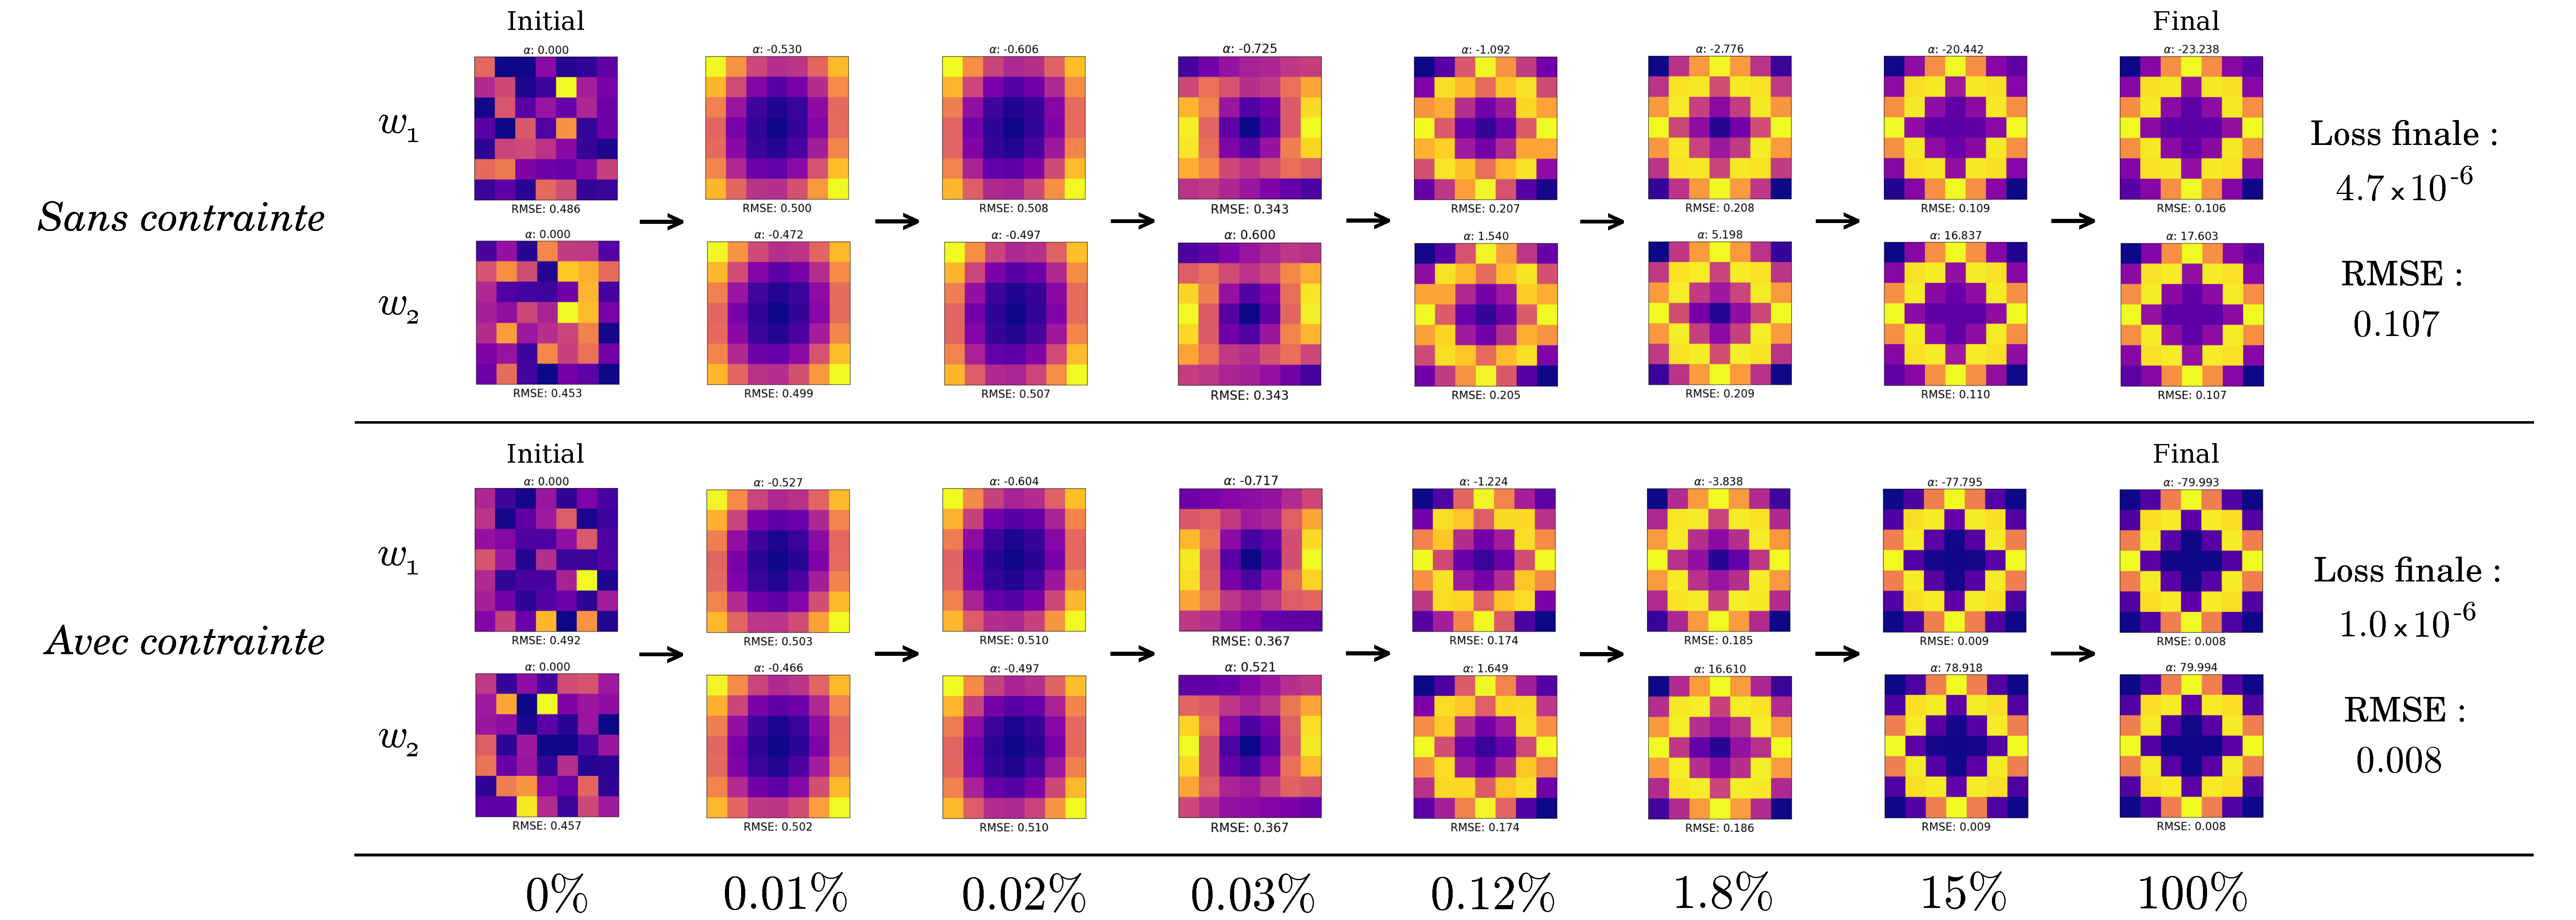
\includegraphics[width=1.00\linewidth]{parts/3-contributions/C-contraintes_geometriques/figures/k_away.pdf}
    \vspace{-4.0mm}
    \caption{ \centering Évolution de la forme du noyau des deux couches du réseau et de sa \textit{RMSE} en fonction de la progression de l'entraînement (en \% avant l'état final), pour le \textit{complex} et l'ouverture sur la banque MNIST, avec et sans la contrainte $C_\text{away}$.}
    \label{fig:c_away}
  \end{center}
\end{figure}


\vspace{-1.6mm}
\noindent À partir de ces résultats, on remarque que cette contrainte permet bien sur cet exemple d'éloigner les deux $\alpha$ de $0$, en les amenant dans ce cas près de $80$ en valeur absolue. On remarque également qu'elle permet ici d'améliorer automatiquement la forme des deux noyaux $w$ du réseau, en les rapprochant davantage de la structure cible (les artéfacts violets au centre et aux bords des noyaux sont réduits), avec une valeur de \textit{RMSE} bien plus faible, et cela simplement grâce à cet éloignement des $\alpha$. La valeur de la \textit{loss} est également plus faible, donc les prédictions sont meilleures grâce à cette contrainte. \\

\vspace{-0.2mm}
Cette contrainte semble efficace lorsque les noyaux $w$ convergent initialement, sans contrainte, vers une forme proche de celle de la fonction structurante cible, et que les paramètres de contrôle $\alpha$ associés sont encore relativement proches de $0$ mais bien du signe espéré et opposé pour les opérations cibles d'ouverture et de fermeture.
Cependant, après différentes expériences réalisées, cette métrique ne semble fonctionner que moyennement pour les expériences qui sont originellement des échecs sans cette contrainte, et pour lesquelles les paramètres $\alpha$ des deux couches du réseau ont le même signe. C'est le cas par exemple de l'expérience avec \textit{adiag} pour l'ouverture et la banque MNIST, pour laquelle $C_\text{away}$ ne permet pas l'éloignement des $\alpha$.


%%% A chaque fois, faire deux comparaisons (schéma de l'évolution du filtre sur plusieurs périodes) : l'une sans la contrainte (prendre un truc qui converge mal), l'autre avec (prendre un truc qui converge bien) !


\newpage

\noindent \textbf{b. Erreur sur l'éloignement opposé}\\

La seconde métrique de contrainte sur les paramètres de contrôle $\alpha$ (ou $p$) est l'erreur sur leur éloignement opposé, notée $C_\text{awayOPP}$. Elle considère deux couches morphologiques en tant que couple, et permet d'éloigner les deux paramètres de contrôle associés, $\alpha_1$ et $\alpha_2$, l'un de l'autre dans une direction opposée dans $\mathbb{R}$. Elle est définie pour tout couple $(\alpha_1,\alpha_2) \in \mathbb{R}^2$, avec un paramètre de régularisation contrôlée $\alpha_\text{ctr} > 0$, par : \\
% sur 2 couches !!!

\vspace{-5.0mm}
\begin{equation}
    C_\text{awayOPP}((\alpha_1, \alpha_2), \alpha_\text{ctr}) = 
    \frac{\alpha_\text{ctr}}{\alpha_\text{ctr} - \alpha_1 \alpha_2}
    \label{erreur_awayOPP}
\end{equation}



\vspace{4.5mm}
\noindent Cette métrique est continue et dérivable partout tant que $\alpha_1 \alpha_2 < \alpha_\text{ctr}$. Par expérience, on sait que si $\alpha_1$ et $\alpha_2$ sont du même signe alors qu'ils ne le devraient pas, alors chacun ne dépassera pas $10$ en valeur absolue. Ainsi, pour que l'inégalité présentée soit toujours vraie en pratique, on donnera par défaut $\alpha_\text{ctr} = 100$. \\

\vspace{-1.6mm}
Prenons l'expérience avec \textit{adiag} pour l'ouverture sur la banque MNIST. La figure ci-après montre l'évolution de la convergence des deux noyaux du réseau durant l'entraînement, sans et avec la contrainte $C_\text{awayOPP}$ dans la \textit{loss} (avec $\lambda = 0.01$). Le réseau a toujours un partage de poids doux. On obtient les résultats suivants sur 6 runs. \\


%figure
\vspace{-1.0mm}
\begin{figure}[htp]
  \begin{center}
    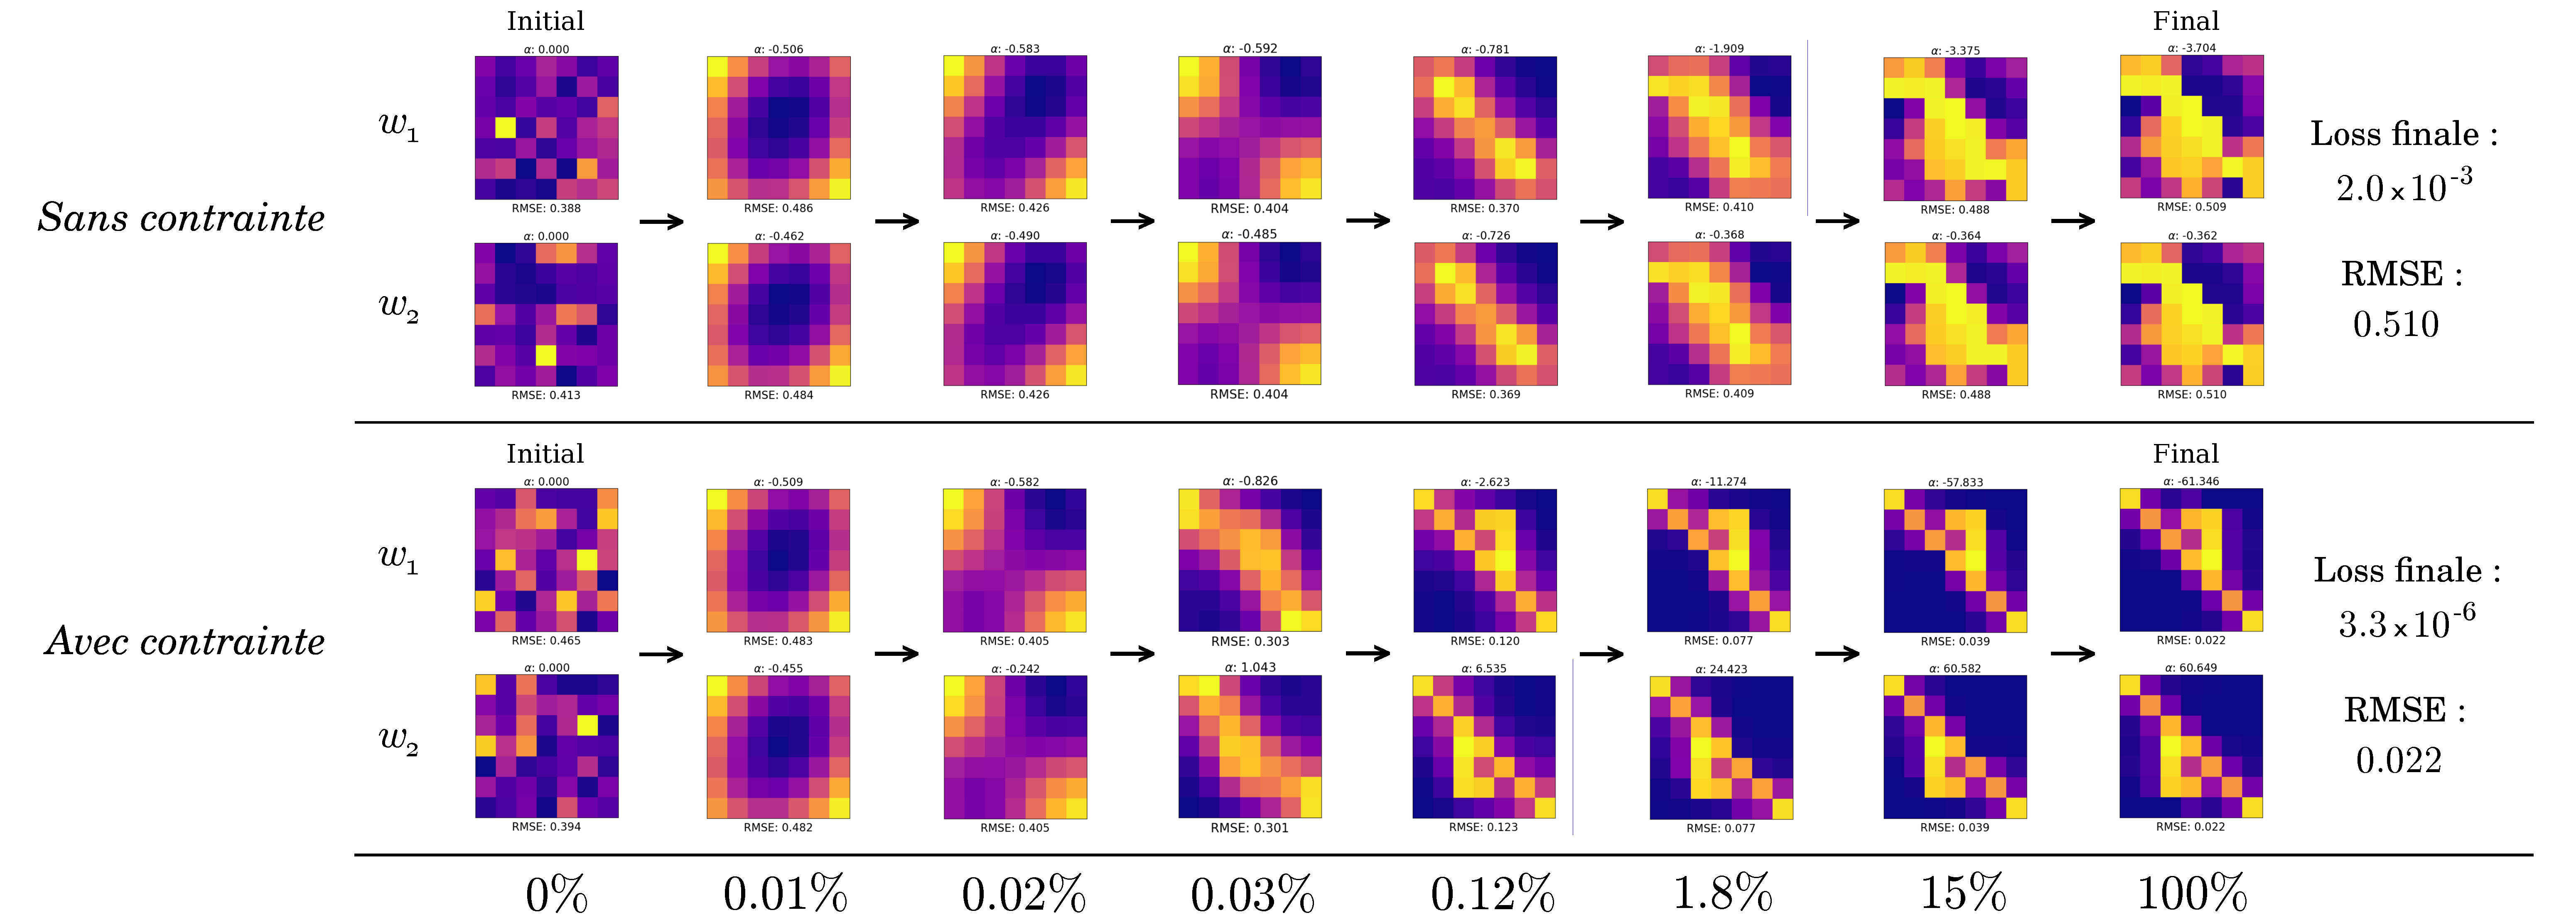
\includegraphics[width=1.00\linewidth]{parts/3-contributions/C-contraintes_geometriques/figures/k_awayOPP.pdf}
    \vspace{-4.0mm}
    \caption{ \centering Évolution de la forme du noyau des deux couches du réseau et de sa \textit{RMSE} en fonction de la progression de l'entraînement (en \% avant l'état final), pour le \textit{adiag} et l'ouverture sur la banque MNIST, avec et sans la contrainte $C_\text{awayOPP}$.}
    \label{fig:c_awayOPP}
  \end{center}
\end{figure}

\vspace{-3.6mm}
\noindent Comme le montrent les résultats de cet exemple, cette métrique est très performante dans les échecs de convergence où les $\alpha$ sont de même signe alors qu'ils ne le devraient pas. Cependant, il faut garder à l'esprit le fait que cette métrique ne peut être utilisée que si on sait à priori que les deux $\alpha$ doivent être de signe opposé.
